%このサンプルは過去の先輩が残してくれたものに,一部修正を加えたものです.


\documentclass[a4paper, twoside]{jarticle}
% a4paper : A4のサイズに設定
% twoside : 偶数/奇数ページで異なるレイアウト,bookのデフォルト.

\usepackage{tani_resume} % 卒論用
\usepackage{epstopdf}
\usepackage{graphicx}
\usepackage{ascmac} % レイアウトを綺麗にする
\usepackage{comment} % 複数行のコメントを使用できる

% 先輩方が全員記述しているため,記述した,検索しても用途が不明
% --- ここから ---
\alignbeforeskip -5mm
\alignafterskip -5mm
\eqnarraybeforeskip -5mm
\eqnarrayafterskip -5mm
\makeatletter
\newenvironment{figurehere}
  {\def\@captype{figure}}
  {}
\makeatother
% --- ここまで ---

\jptitle{千代田区空散歩アプリ「ちよダッシュ!」の開発} % タイトル
\etitle{} % 空白で構わない
\jpauthor{岩田匡裕・高山泰征・安田貴裕} % 名前
\eauthor{Masahiro Iwata, Taisei Takayama, Takahiro Yasuda} % 名前(ローマ字)
\course{谷聖一 研究室} % {谷聖一 研究室}で良い
\year{元} % 自分たちの代の年度
%多分これを見る頃には平成じゃなくなっているので誰かtani_reusme.styを変更する必要あり
% \rhead{\date{}}
% \date{\today}

\abstract{ % 概要
本演習では,iOS・Android に対応した千代田区散歩アプリ「ちよダッシュ!」のコンセプトとプロトタイプを基に,改良・改善を加えた正式版の開発とリリースを行なった.
}

% 右上に最終更新時刻を表示する,バックアップを見返す際に便利
% 先輩方は完成時にはコメントアウトしている
% \compheading % 最終更新時刻

% \date{\now}


\begin{document} % 文書(開始)
\maketitle % タイトルを表示する
\begin{multicols}{2} % 2段落にする(開始)
\setcounter{page}{1} % ページ開始番号

% はじめに
\section{はじめに}

\subsection{人文学とデジタル・ヒューマニティーズ}
%%%人文科学とは%%%
『人文学は,「人間」とは何かということを様々な媒体や方法によって追求する,人間研究の基礎学』(\cite{huma})である.\par
%%%デジタル%%%
近年,情報通信技術の発達などによりデジタル技術の発達がみられる.
%デジタル・ヒューマニティーズ
デジタル技術は,「人類の知的資源の保存,研究,発信の方法を大きく変えて,情報社会の新しい知識基盤を形成しています.この変化に対応すべく,デジタル媒体による学術資料のアーカイブ構築,文化コンテンツの分析,学術成果の公開や展示の方法などを,文系・理系の枠組みを横断して研究するデジタル・ヒューマニティーズの動きが世界的に拡がっています」(\cite{digihumu1}).\par

デジタル・ヒューマニティーズとは,情報学的手段を用いて人文学的問題を模索することで,人文学的問題をきっかけとした新たな情報学の分野を切りひらき,新しい知識や視点を得ることを目指している研究領域である(\cite{digihumu2}).

\subsection{千代田学}
千代田区では,以下に引用するように,区内の大学と「千代田の魅力創出と発展という目的」で提携している.『千代田区には,日本でも有数の学校等が数多く在籍し,多くの教育文化施設が立地するなど,町全体が知識・文化の発信地となっています.区内の大学においては,特色のある高度な教育や研究,産学連携など開かれた大学としての取り組みを行っており,区は 11 校の大学と「千代田区内大学と千代田区の連携協力に関する基本協定」を結んでいます(\cite{digi4})』.
千代田区は,その提携事業の一つとして,区内にある大学が千代田区の様々な事象を多様な切り口で調査・研究することを「千代田学」と名付け,その定着と発展を目指し,必要となる経費の一部を区が補助する「千代田学」提案制度を平成16年度より行っている.令和元年度「千代田学」提案制度に,日本大学からは「千代田ヴァーチャル時空散歩アプリちよダッシュ!の充実と展開」が採択されている(\cite{digi5}).

\subsection{千代田区と日本大学}
千代田区は,1947年(昭和22年) 3月15日に麹町区と神田区が合併して誕生した.東京23区のほぼ中央に位置し,区の中央には,皇居のある「千代田区千代田」があり,千代田区全体の約12\%が皇居の緑地となっている.また,1457年に築城された江戸城は「千代田城」とも呼ばれ,千代田区の名称の由来となっている(\cite{digi1}).

\subsection{参加プロジェクト}
副題ですね

% \subsection{何か書く}
% 副題ですね


\section{先行研究}


\subsection{江戸・東京WebGISについて}
日本大学文理学部では平成22年度の文部科学省私立大学戦略的研究基盤形成支援事業(\cite{monka})において,東アジアにおける都市形成プロセスの統合的把握とそのデジタル化をめぐる研究のプロジェクトの研究の一環として,いくつかの研究成果を公開 している.その一つとして「江戸・東京WebGIS」が公開されている.「江戸・東京WebGIS」は、Google Map上に古地図や文学テキストならびに言語資料を配置し,日本語日本文学の観点から近世・近代・現代を透かし見ることで江戸・東京圏を再構築することを目指したWebアプリである.現代の地図に近世期の地図「江戸切絵図」(1849-52年刊行)や近代期地図「東京市全図」(1907年刊行)を重ね合わせ,これら古地図の透過表示することができ,近世・近代・現代を透かし見ることができる.このような重層的地図に,近世・近代・日本語に関連する資料を配置している.(\cite{webgis_gaiyo})

\subsection{江戸・東京ものがたりについて}
また,「江戸・東京WebGIS」はスマートフォンでも閲覧することができていたものの,データ量が多く,十分に動作が重いなどの問題があり,不便であった.そのため,スマートフォンでの使用に特化したプロトタイプアプリ「江戸・東京ものがたり」が昨年度の卒業演習により作成された(\cite{houkokusyo_30}).このアプリは今年度の演習において正式版を作成し,一般公開を目指しているためGoogle PlayストアとApp Storeで一般公開をするための審査中である.

\subsection{ちよダッシュ!について}
平成30年度の「千代田学」調査・研究(\cite{tiyokenkyu})においてWebGISを用いた千代田ヴァーチャル時空散歩アプリの構築を研究テーマとし,「千代田ヴァーチャル時空散歩」ができるプロトタイプアプリの構築を目的(\cite{tiyodagaku_houkokusyo})として,本アプリが作成された.

ちよダッシュ!は「江戸・東京WebGIS」サイトをベースとした地図上のピンの場所を巡る位置情報アプリである.散歩の友としてこのアプリを利用し誰でも楽しめることをコンセプトとしており,千代田区に足を運んでいただき,千代田区に興味をもってもらうことを目的として作られた.

\subsection{昨年度のちよダッシュ!}
先ほど述べたようにちよダッシュ!は昨年度から作成が始まっているアプリであり,昨年度はコンセプトとプロトタイプアプリ作り,今年度は開発と一般公開とそれぞれ別々なことを演習として取り組んでいる.昨年度のちよダッシュ!では主にコンセプトとプロトタイプアプリを作り,コンセプトは「散歩の友としてこのアプリを利用し誰でも楽しめること」と決まった.またプロトタイプの主な実装機能としてGoogle Maps 上での資料閲覧機能とスタンプラリー機能が追加された.


\section{本演習}

% \subsection{今年度のちよダッシュ!}
% 次の内容の副題ですね

\subsection{今年度のちよダッシュ!}
今年度のちよダッシュ!は昨年度のプロトタイプをベースに機能を拡張した.

\subsection{スプラッシュ画面}
スプラッシュ画面
デザインは外部に依頼して作成
千代田区がシンボルにしている「松・桜・白鳥」と
古地図を用いている.(図 1 参照)
\begin{figurehere}
\begin{center}
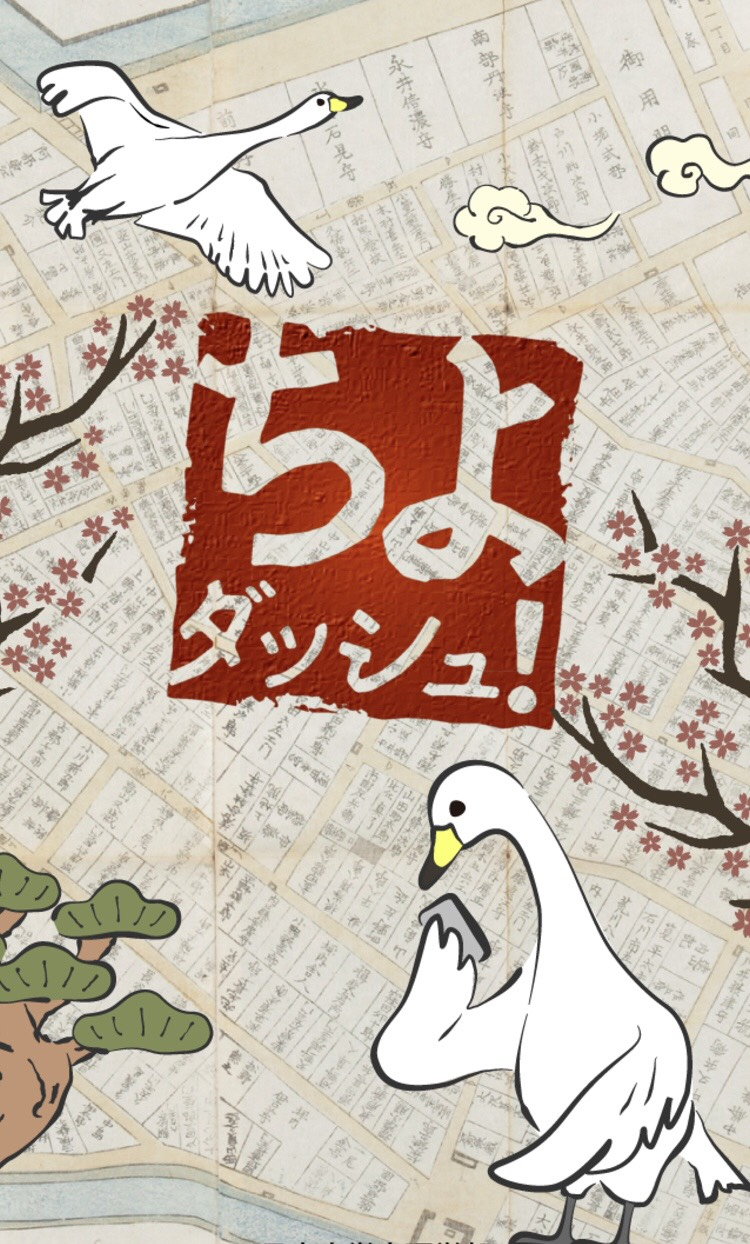
\includegraphics[bb=30 50 550 1300,width=3cm]{./image01.jpg}%%750*1334(100%)でスクショ[大きさ 横 縦,width]
\end{center}
\caption{スプラッシュ画面}\label{fig:1}
\end{figurehere}

\subsection{利用規約同意画面・利用規約の任意確認}
利用規約を日本語か英語かを上のボタンから切り替えができる.今後表示しないにチェックを入れると次のアプリ起動時から利用規約画面が表示されなくなる.(図 2,3 参照)
\begin{figurehere}
\begin{center}
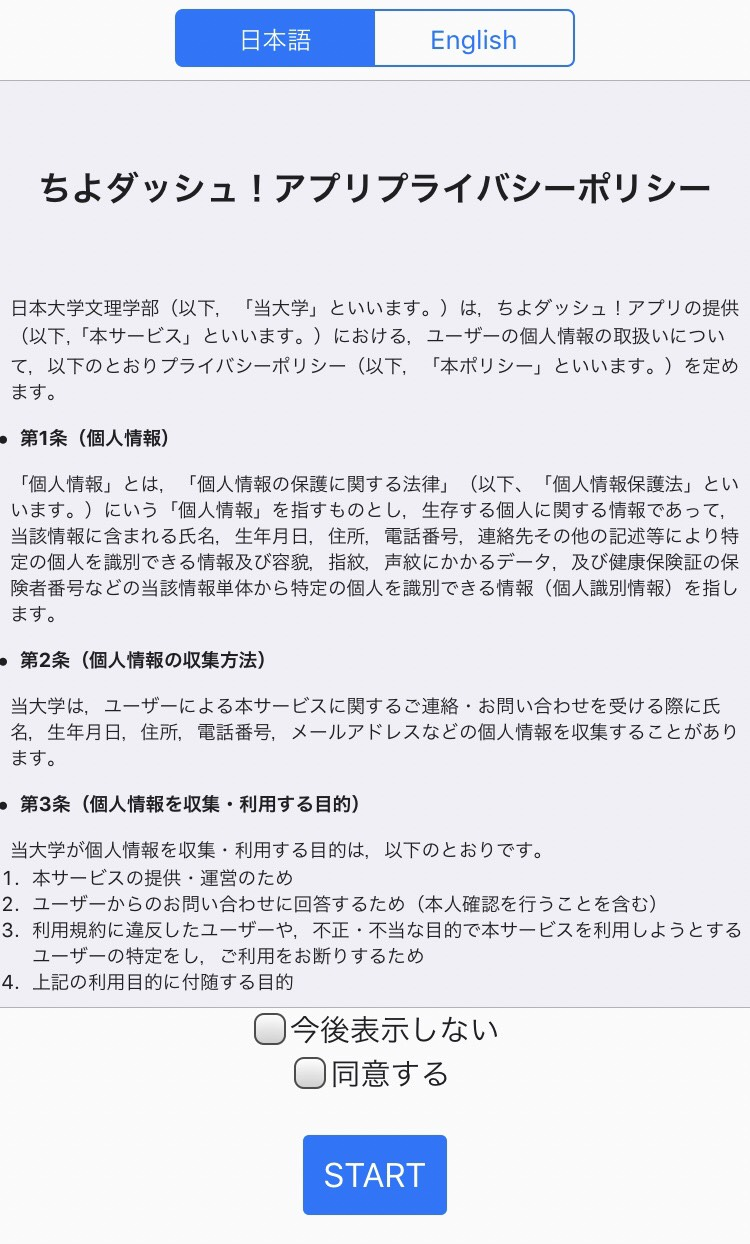
\includegraphics[bb=30 50 550 1300,width=3cm]{./image02.jpg}%%750*1334(100%)でスクショ[大きさ 横 縦,width]
\end{center}
\caption{利用規約画面 日本語}\label{fig:2}

\begin{center}
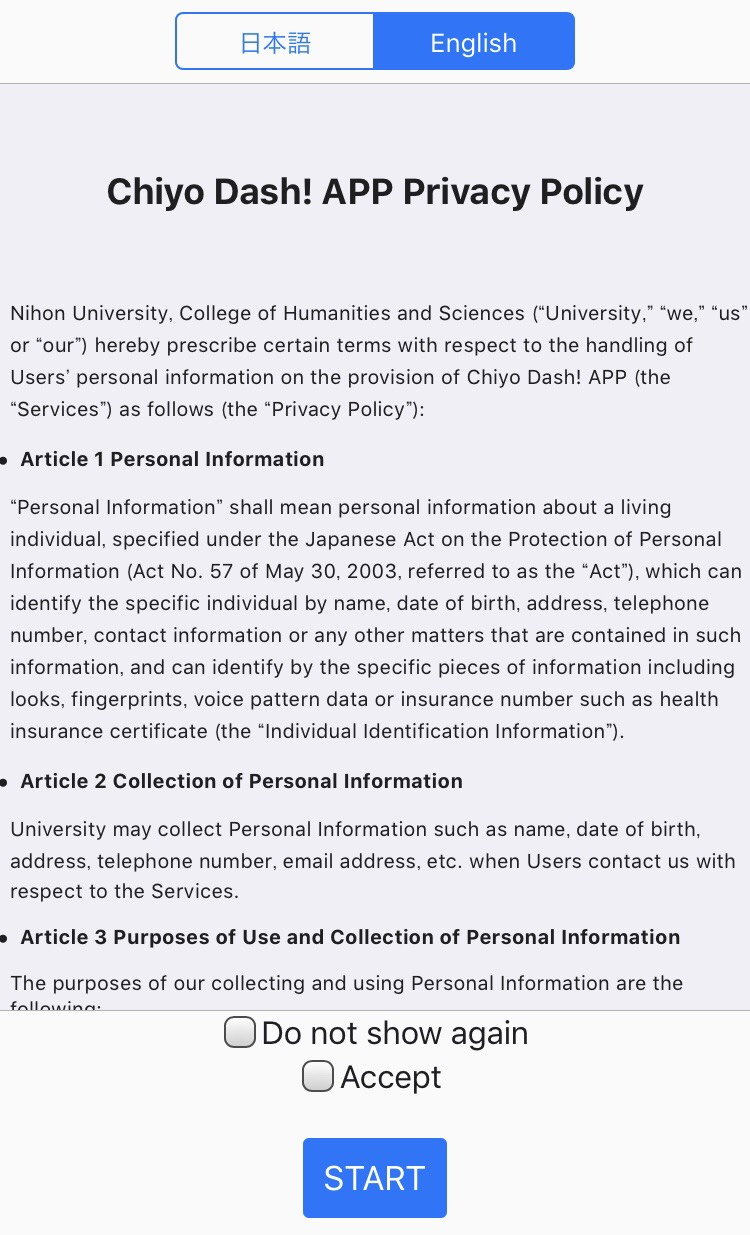
\includegraphics[bb=30 50 550 1300,width=3cm]{./image03.jpg}%%750*1334(100%)でスクショ[大きさ 横 縦,width]
\end{center}
\caption{利用規約画面 英語}\label{fig:3}
\end{figurehere}
% また同意するにチェックを入れないとアラートが表示される.

% \begin{center}
% 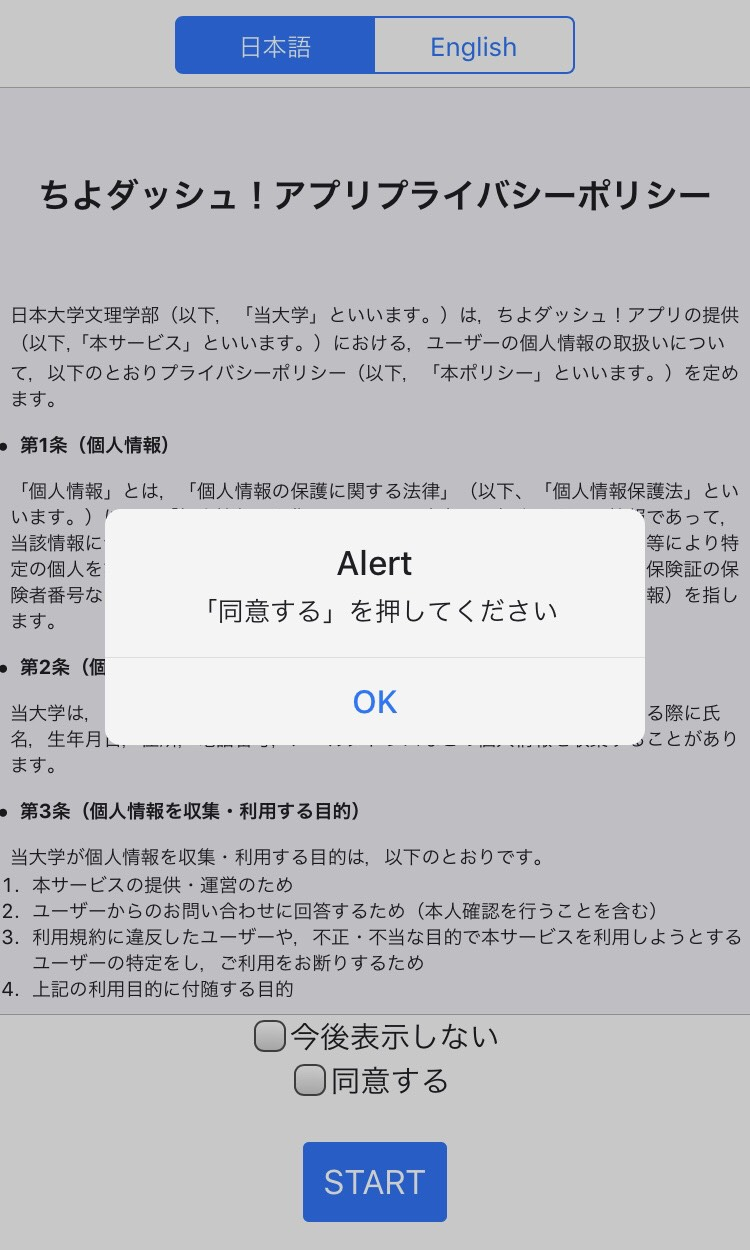
\includegraphics[bb=30 50 550 1300,width=3cm]{./image04.jpg}%%750*1334(100%)でスクショ[大きさ 横 縦,width]
% \end{center}
% \caption{利用規約画面3}\label{fig:4}
% \end{figurehere}

\subsection{スタンプ獲得の有無によるピン表示の変更}
スタンプを取得するとピンを黒点のあるものから黒点のないピンの画像に変えることにより,ユーザがどの場所を訪れたのかがわかるようにした.(図 4,5 参照)
\begin{figurehere}
\begin{center}
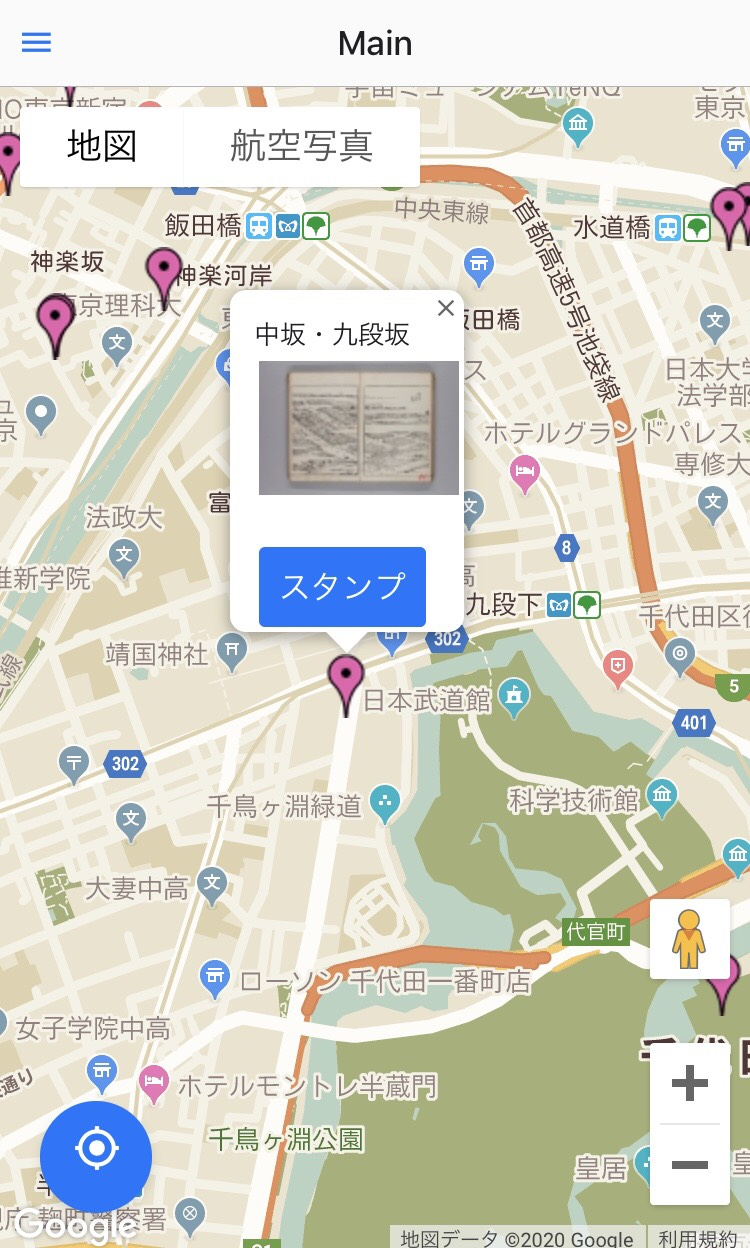
\includegraphics[bb=30 50 550 1300,width=3cm]{./image05.jpg}%%750*1334(100%)でスクショ[大きさ 横 縦,width]
\end{center}
\caption{スタンプ取得前}\label{fig:5}

\begin{center}
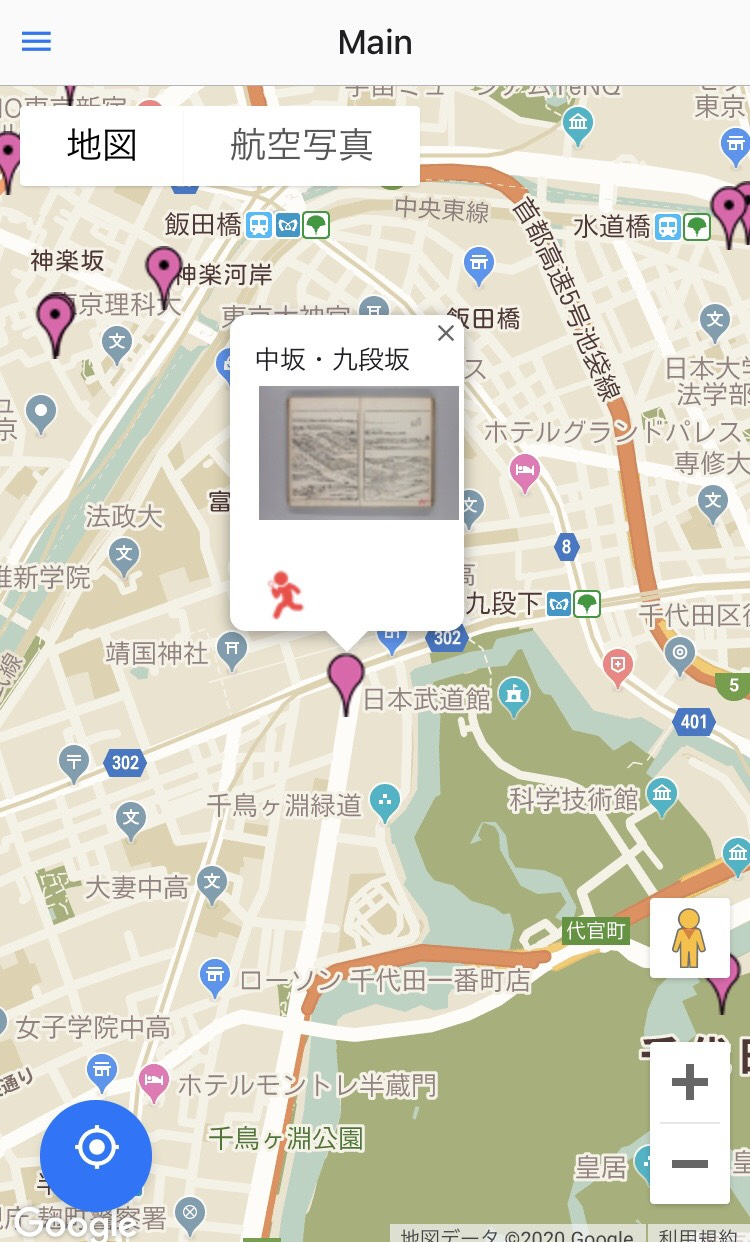
\includegraphics[bb=30 50 550 1300,width=3cm]{./image06.jpg}%%750*1334(100%)でスクショ[大きさ 横 縦,width]
\end{center}
\caption{スタンプ取得後}\label{fig:6}
\end{figurehere}

\subsection{画像資料の追加・ダイアログ表示}
本文が長い名所や,画像付きのものはダイアログを使用して表示を複数に分けた.(図 6,7 参照)
\begin{figurehere}
\begin{center}
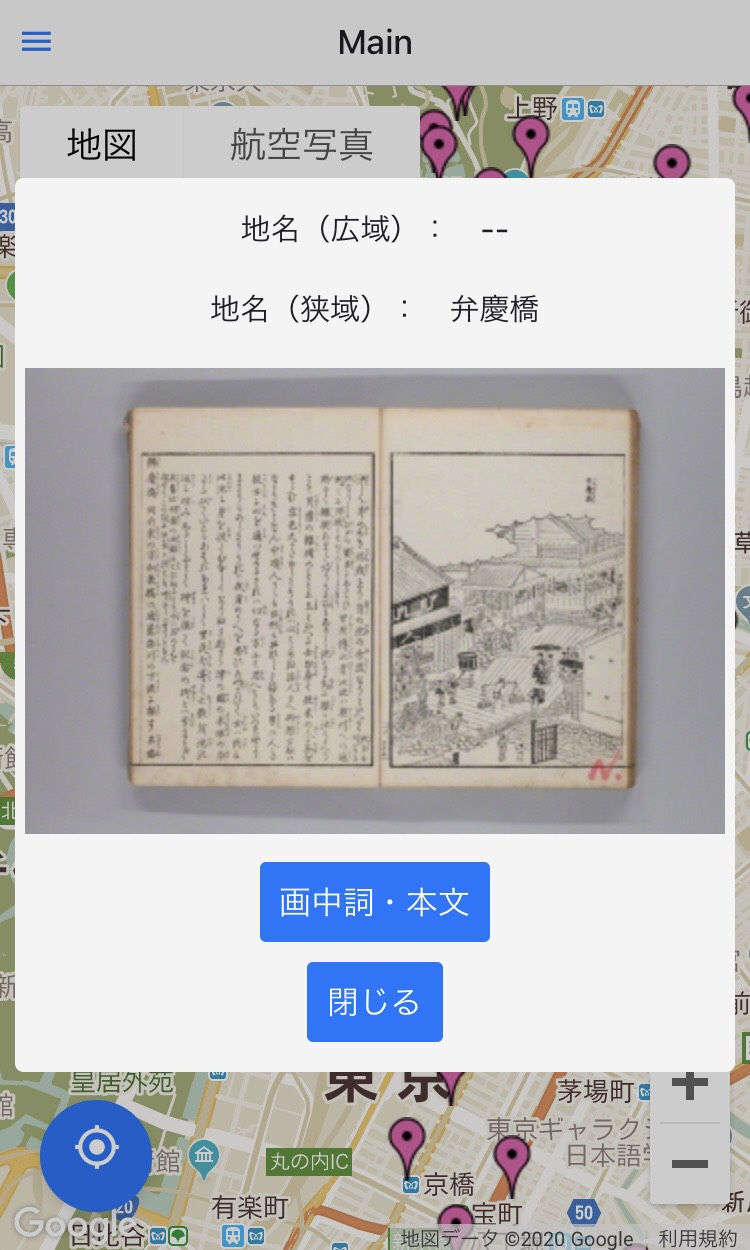
\includegraphics[bb=30 50 550 1300,width=3cm]{./image07.jpg}%%750*1334(100%)でスクショ[大きさ 横 縦,width]
\end{center}
\caption{ダイアログ表示1}\label{fig:7}
\end{figurehere}

\begin{figurehere}
\begin{center}
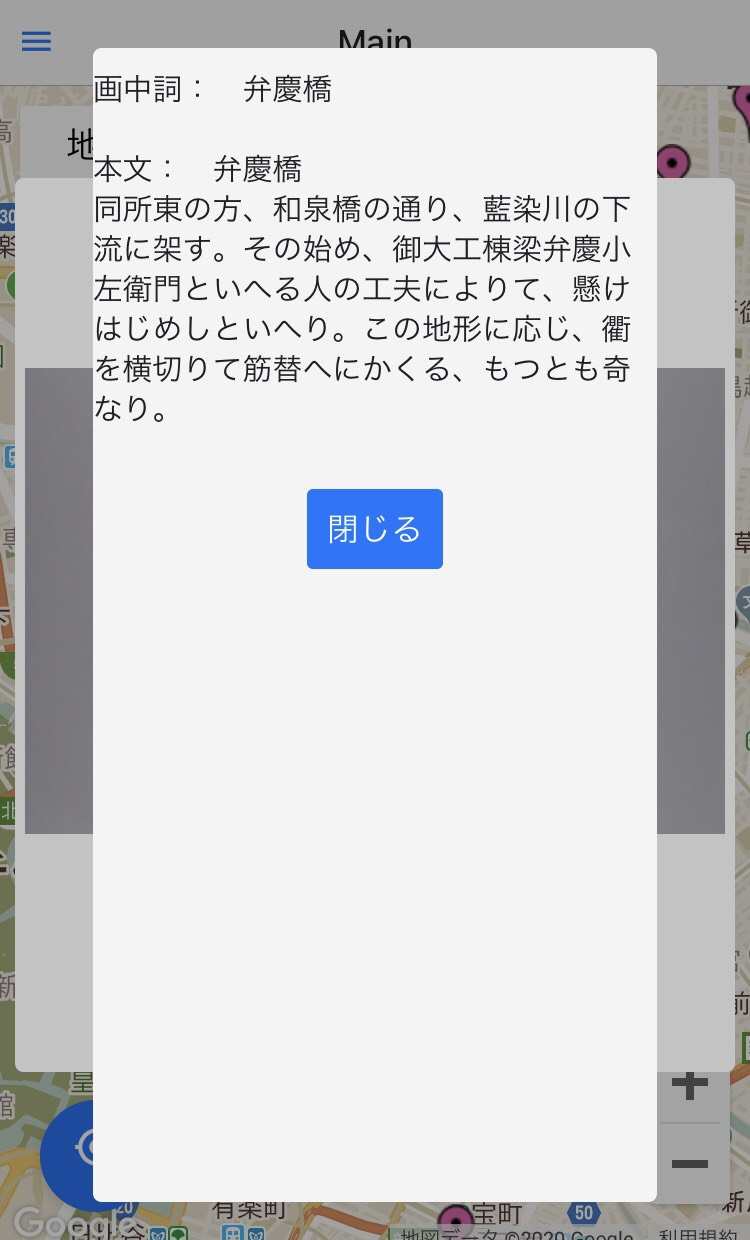
\includegraphics[bb=30 50 550 1300,width=3cm]{./image08.jpg}%%750*1334(100%)でスクショ[大きさ 横 縦,width]
\end{center}
\caption{ダイアログ表示2}\label{fig:8}
\end{figurehere}

\subsection{スプリッター・ステータスバー}
画面左上の三本線のボタンを押すと画面左からスプリッターが表示される.複数のピン選択項目があり,表示させたいピンの項目を選択することで地図上に選んだ項目のピンを表示することができる.(図 8 参照)\par
また,下にスクロールすることでそれぞれのピンの取得数を項目ごとに棒グラフと共に確認することができる.\par
一番下には利用規約を閲覧するボタンを実装し,いつでも利用規約を確認することができる.(図 9 参照)
\begin{figurehere}
\begin{center}
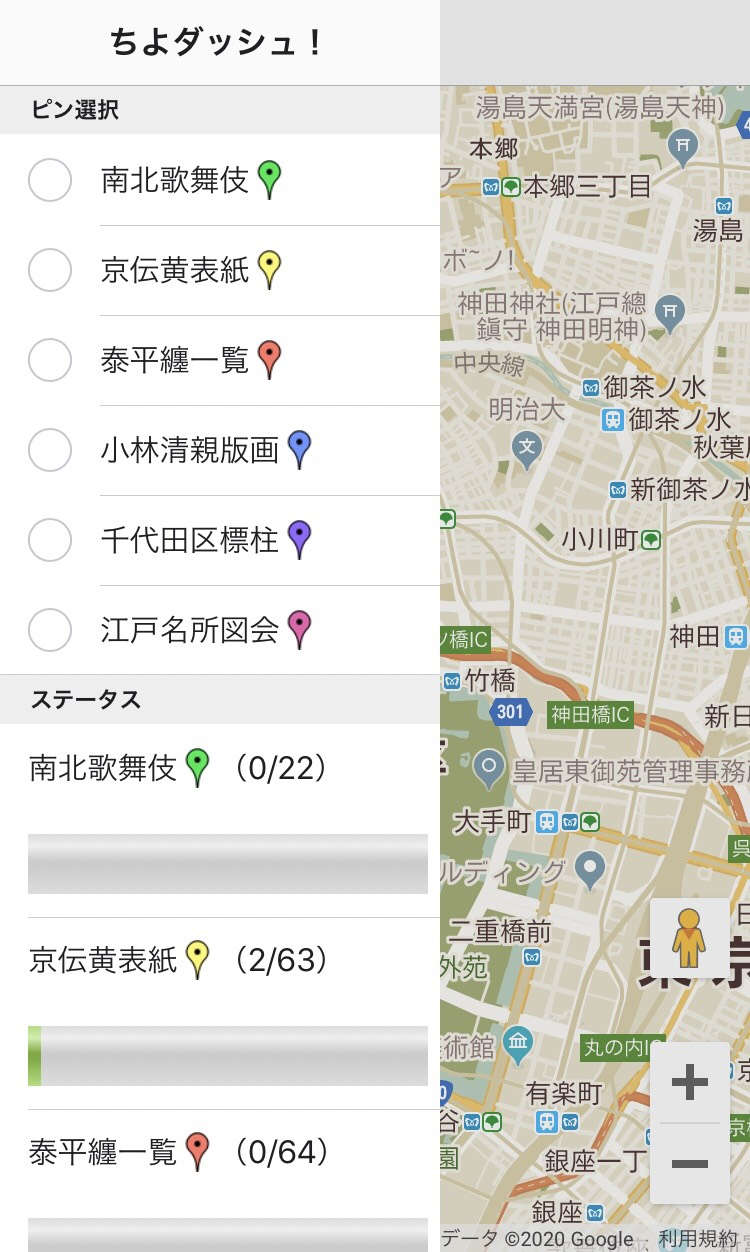
\includegraphics[bb=30 50 550 1300,width=3cm]{./image09.jpg}%%750*1334(100%)でスクショ[大きさ 横 縦,width]
\end{center}
\caption{スプリッター・ステータスバー}\label{fig:9}
\end{figurehere}

\begin{figurehere}
\begin{center}
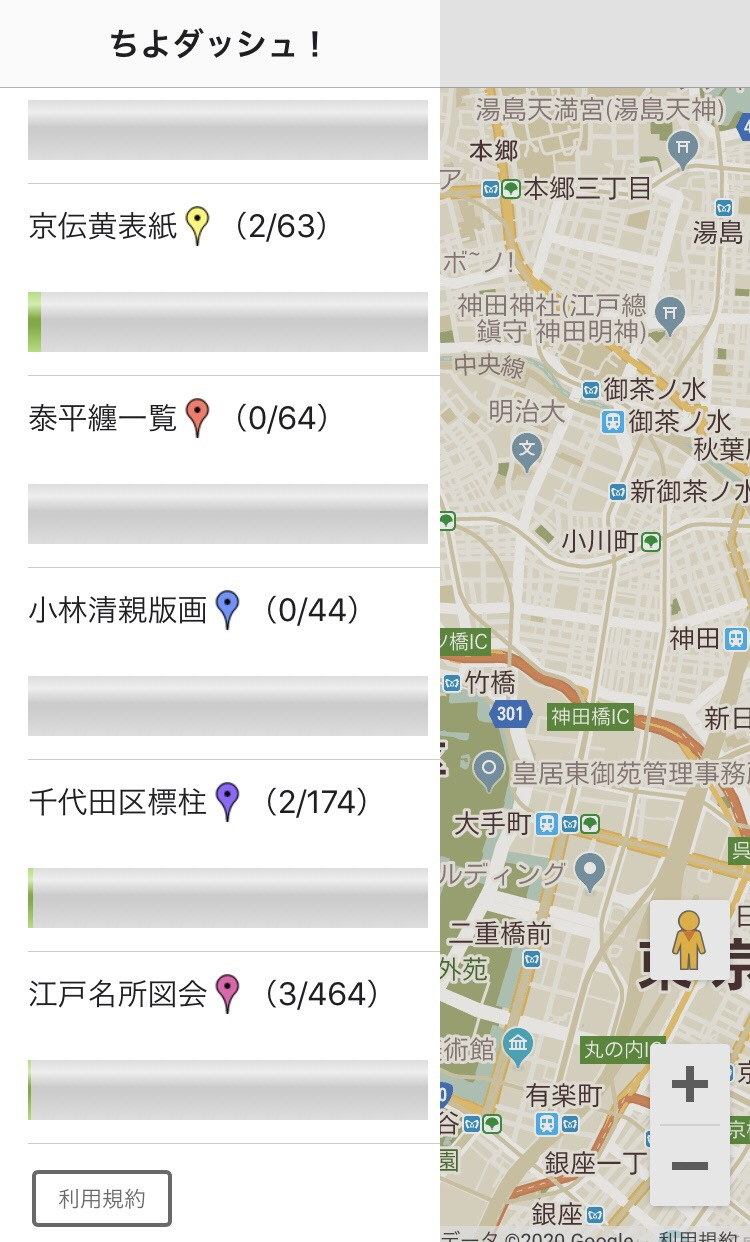
\includegraphics[bb=30 50 550 1300,width=3cm]{./image10.jpg}%%750*1334(100%)でスクショ[大きさ 横 縦,width]
\end{center}
\caption{スプリッター・ステータスバー2}\label{fig:10}
\end{figurehere}


\subsection{トースト機能}
ユーザが名所のスタンプを押す時に名所の100m以内にいない場合,スタンプが押せず画面下から警告が表示される.(図 10 参照)
\begin{figurehere}
\begin{center}
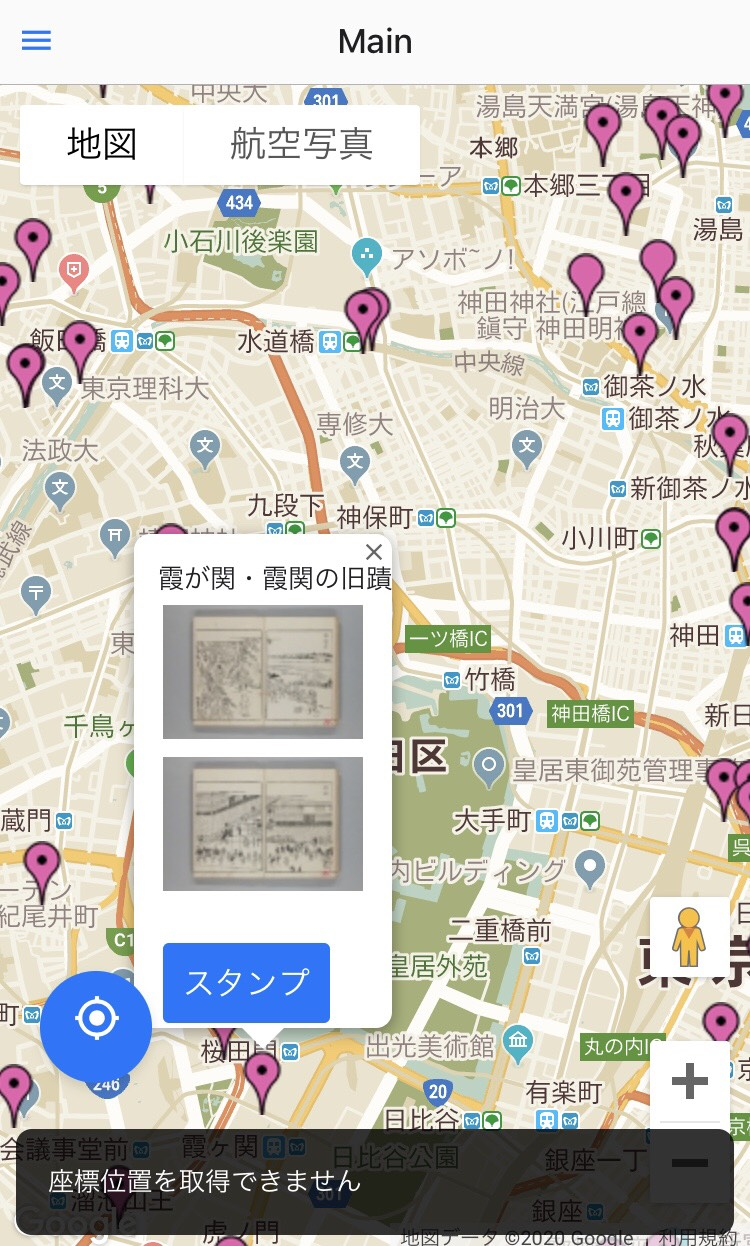
\includegraphics[bb=30 50 550 1300,width=3cm]{./image11.jpg}%%750*1334(100%)でスクショ[大きさ 横 縦,width]
\end{center}
\caption{トースト}\label{fig:11}
\end{figurehere}

\subsection{現在地自動取得}
アプリ起動時に自動的に現在地を取得する.また画面左下の青いボタンを押すと任意で現在地を取得することができるようになっている.

\subsection{ピン表示時のアニメーションの追加}
ユーザがピンを表示する際にピンが上から落ちてくるようなアニメーションを追加した.

\subsection{使用した API}
マップの表示,テキスト情報の表示にあたり「Google Maps Platform」を使用した.Google Maps Platform とは,Google 社が提供している高機能で世界中の地図データを扱っている Google Maps を,さまざまなサービスで利用できるようにしたもので,Android や iOS 向けアプリや Web サービスに Google Maps を使用することができる ([10]).これを利用することで,マーカー,ライン,色,ポリゴン,画像をカスタマイズして独自の地図を作成することができる.

\subsection{アプリの開発環境}
本演習では Monaca を用いてアプリ開発を行った.Monaca とは,HTML5,JavaScript などの Web 標準言語でモバイルアプリ開発を行うことができるクラウドベースの開発プラットフォームである.ブラウザ上でコーディングができ,UI のライブプレビューなどの機能を提供している

\subsection{データベース管理機能}
本演習において Monaca を用いるにあたり,データベース管理機能については Monaca との連携が容易であるニフクラ mobile backend を利用した.ニフクラ mo-bile backend とは,文学テキストや言語資料をクラウド上で管理できるクラウドサービスである.会員管理・認証やデータベース管理などの機能も備わっているため,スマートフォンアプリでよく利用される汎用的な機能を導入することができる.

\subsection{ステータスデータ保存方法}
本演習ではLocalStorageを用いてステータスデータを端末に保存した.LocalStorageとは,HTML5から追加された新機能で,javascript利用することでユーザーのデータをwebブラウザ(ローカル環境)に保存することができる仕組みである.

\subsection{アプリとデータ通信に関する関係図}
アプリ起動時にニフクラからピンに関する情報(タイトル・座標・画像データのURL)を取得する.画像データのURLは江戸・東京WebGISのものである.ユーザがスタンプを押すとその情報はステータス情報としてLocalStorageに保存される.LocalStorageに保存することにより,次回起動時にもユーザのステータス情報を引き継いで使うことができる.また,ピン情報はニフクラから取得しているので,アプリのアップデートなしに新規のピンを追加することができる.(図 11 参照)
\begin{figurehere}
\begin{center}
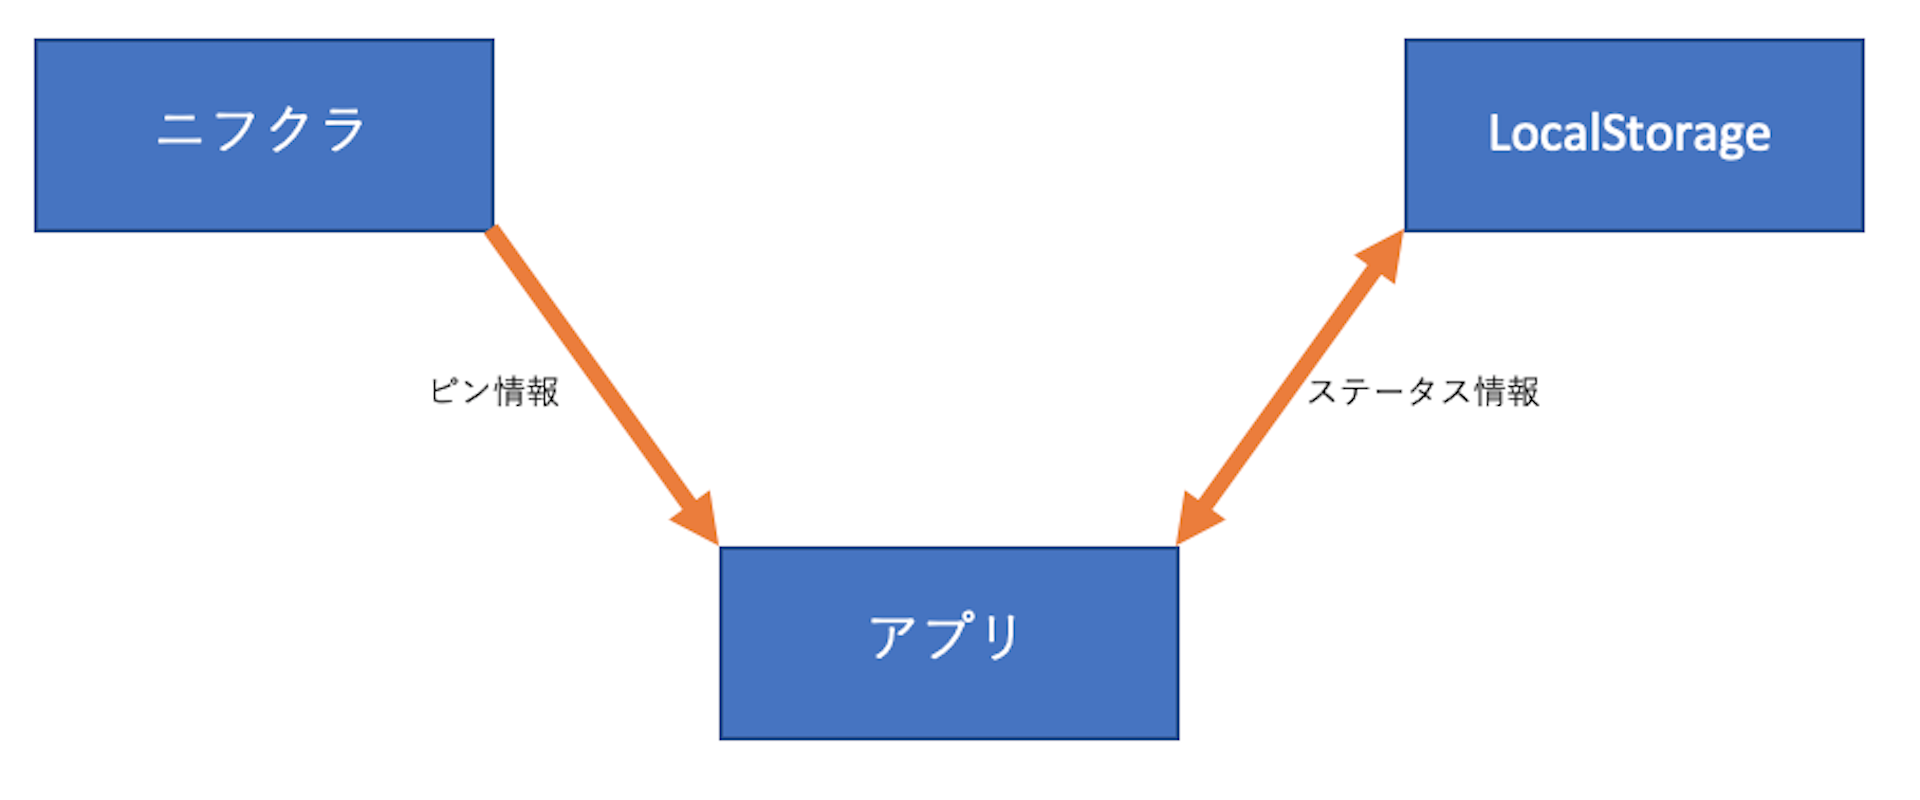
\includegraphics[bb=30 100 550 500,width=3cm]{./image12.png}%%750*1334(100%)でスクショ[大きさ 横 縦,width]
\end{center}
\caption{アプリとデータの関係図}\label{fig:12}
\end{figurehere}


\section{終わりに}
本演習では,昨年度のちよダッシュ!のコンセプトとプロトタイプを基づき、改良・改善を加えた正式版の開発とリリースを行った.開発する上で,Monaca,ニフクラmobile backend,LocalStorage,Google Maps Platform を使用し,昨年度のちよダッシュ!にステータス機能を加えることによりゲーム性を高め,GUIを改善することによりアプリを利用しやすくした.また,ピンの種類を増やすとともにピン詳細の画像を表示することで街歩きをより楽しめるようにした.\par
本演習においての課題は,一般公開をしてユーザに使用してもらった感想などを基づき,より使いやすいアプリに改良することである.



\end{multicols} % 2段落にする(終了)
\vspace{1cm}
% multicols を end したあとに参考文献
\begin{thebibliography}{99}

\bibitem{huma}文部科学省 人文学及び社会科学の意義・役割・目的について\par
http://www.mext.go.jp/b\_menu/shingi/gijyutu/gijyutu4/015/siryo/attach/1343073.htm (参照:2020-2-06)

\bibitem{digihumu1}東京大学大学院横断型教育プログラム デジタル・ヒューマニティーズ\par
http://dh.iii.u-tokyo.ac.jp/ (参照:2020-2-06)

\bibitem{digihumu2}国立情報学研究所(NII) 北本 朝展 デジタル・ヒューマニティーズ\par
http://agora.ex.nii.ac.jp/\~kitamoto/research/dh/ (参照:2019-2-12)

\bibitem{digi1}千代田区 区の起こり・由来\par
https://www.city.chiyoda.lg.jp/koho/kuse/gaiyo/yokoso/okori.html (参照:2019-2-12)

\bibitem{digi4}千代田区役所 区内大学,専修・各種学校等と区の連携協力 平成16年度〜「千代田学」提案制度\par
https://www.city.chiyoda.lg.jp/koho/kurashi/volunteer/renke/index.html (参照:2020-2-06)

\bibitem{digi5}「千代田学」調査・研究実績報告書\par
https://www.city.chiyoda.lg.jp/koho/kurashi/volunteer/tean-ichiran.html (参照:2020-2-06)

\bibitem{monka}文部科学省私立大学戦略的研究基盤形成支援事業\par
https://www.mext.go.jp/component/a\_menu/education/detail/\_\_icsFiles/afieldfile/2010/04/23/1267810\_3\_1.pdf (参照:2020-2-06)

\bibitem{webgis_gaiyo}日本語日本文学半プロジェクト江戸・東京WebGIS概要\par
http://dep.chs.nihon-u.ac.jp/japanese\_lang/nichigo-nichibun/\#content\_03 (参照:2020-2-06)

\bibitem{houkokusyo_30}平成30年度千代田学研究成果報告書WebGISを用いた千代田ヴァーチャル時空散歩アプリの構築日本大学 田中ゆかり\par
https://www.city.chiyoda.lg.jp/koho/kurashi/volunteer/documents/nihon30-1.pdf (参照:2020-2-06)

\bibitem{tiyokenkyu}「千代田学」調査・研究実績報告書\par
https://www.city.chiyoda.lg.jp/koho/kurashi/volunteer/tean-ichiran.html (参照:2020-2-06)

\bibitem{tiyodagaku_houkokusyo} WebGISを用いた千代田ヴァーチャル時空散歩アプリの構築 日本大学・田中ゆかり\par
https://www.city.chiyoda.lg.jp/koho/kurashi/volunteer/documents/nihon30-1gaiyo.pdf (参照:2020-2-06)

\bibitem{api} 「Google マップを使ってみよう!」\par
https://www.zenrin-datacom.net/business/media/g001/index.html(参照:2020-2-06)

% \bibitem{} (参照:2020-2-06)

% \bibitem{} (参照:2020-2-06)

\end{thebibliography}

\end{document} % 文書(終了)
